\subsection{Small-scale evaluations}
\label{sec:small-scale}

% Topology description
To assess baseline quality of the designed Interest flooding attack mitigation methods, we evaluated them first using a simplistic small-scale binary tree topology (Fig.~\ref{fig:small-scale}).
All links in this topology were assigned 10~Mbps bandwidths with randomized propagation delays from the range from one to ten milliseconds.
Both legitimate users and attackers were placed only on leaf nodes (red), each expressing Interests towards a single producer placed at the root of the tree. 
% Alex: should we mention that?
The main reason to chose a binary tree topology was that it represents one of the worst cases to defend against flooding DDoS attacks.
That is, sharing of the network links exponentially increases as decreasing level of the binary tree.

\begin{figure}[htbp]
  \centering
  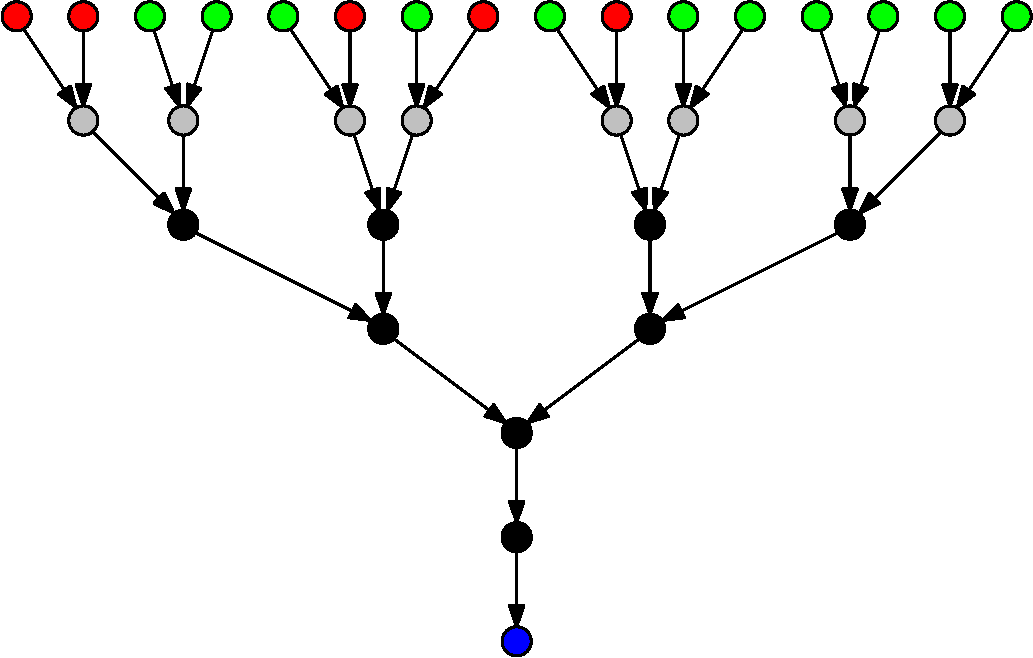
\includegraphics[scale=0.2]{topo-tree-evil-5-good-0-producer-gw}
  \caption{Small-scale binary tree topology}
  \label{fig:small-scale}
\end{figure}

% in 10 independent runs of each simulation, where we randomized position of the adversaries along the legitimate users.   In all runs, the total number of legitimate and malicious uses were fixed, meaning that when we increase number of attackers, we decrease the number of legitimate users.   

\subsubsection{Network reaction to the attack}

The first set of experiments aims to evaluate reaction of the network and Interest flooding attack mitigation methods mechanisms under a moderate-level DDoS attack.
For this purpose, we simulated four different network scenarios, in which all routers implements the same attack mitigation algorithm, either token bucket with per interface fairness, satisfaction-based Interest acceptance, or satisfaction-based pushback (Section~\ref{sec:design}).

For each network scenario we performed ten independent simulation runs, where randomly chosen 7 client nodes represent adversaries (compromised users), and the rest 9 client nodes represent legitimate users.
In each run we simulated a 10-minute attack window (total simulation time was 30 minutes, with attack starting at 10-minute mark).

The results for all attack mitigation algorithms and all runs are aggregated in Fig.~\ref{fig:small-scale attack progress}, where Y-axis represents a minimum and maximum range for observed Interest satisfaction percentages among all nodes and all simulation runs.
A short and simplistic summary of the results is that the first two attack mitigation methods do not work at all, and the last two are working quite good.

\begin{figure}[t]
  \centering
  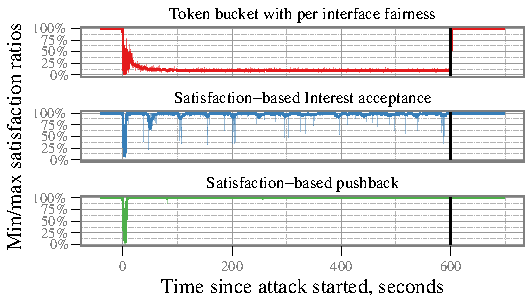
\includegraphics[scale=0.8]{paper-topo-tree/tree-good-0-producer-gw}
  \caption{Satisfaction ratio dynamics during the attack (7 attackers / 9 legitimate)}
  \label{fig:small-scale attack progress}
\end{figure}

\paragraph{\textbf{Simple token buckets}}

{\color{red}Alex: should this discussion be removed or we still want to keep it (as it is referenced later and potentially before)}

Let us take a deeper look on what is happening with the physical limits algorithm.
Essentially, we observe an extremely successful denial of service attack, where attackers almost completely shut down legitimate users from the Data producer (using a relatively small amount of Interests, as physical limits restricts the number of forwarded Intersets!).
This ``success'' can be explained using a simplistic example, illustrated on Fig.~\ref{fig:three router example}, where each router has only one token for Interest forwarding.
In this example we assume that both the legitimate user and the adversary send Interests in about the same time.

\begin{figure}[t]
  \centering
  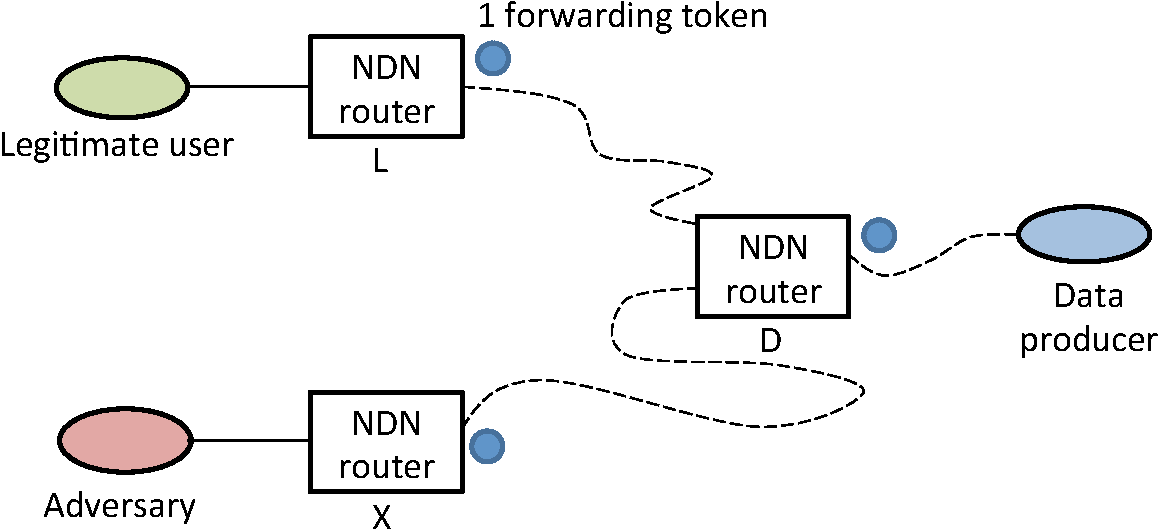
\includegraphics[scale=0.3]{physical-limits-sync-problem}
  \caption{Three-router topology, with one legitimate and one malicious user}
  \label{fig:three router example}
\end{figure}

Both router L and router X will forward the Interests, as both of them have a free token available.
At router A, two cases are possible, either of Interests can arrive first, resulting in a quite different effects.
When legitimate Interest arrives first, then there are no problem. 
Router A will capture the token, forward the Interest, which will be quickly satisfied, releasing the token for future uses.
In the mean time, malicious Interest will be dropped at router A, and router X will release the hold for the token in one second (i.e., after the maximum time Interests are admitted), enabling a new round of competition for router A's resources.

In the case when malicious Interest is sent a little bit earlier, then router A will forward malicious Interests, dropping a legitimate one, and causing ``lock out'' for one second.
In the instant when the token gets released at router X, an adversary is able to push new Interest towards router A, which may arrive in the exact time A's token gets released (assuming an idealistic environment).
As a result, the adversary recaptures router A's token and extends the ``lock out'' for another second, denying service to the legitimate user without sending any massive numbers of Interests.

\paragraph{\textbf{Token bucket with per interface fairness}}

The described problem arises from the clocking effect and can be solved in a number different ways.
Augmenting physical limits algorithms with per-interface fair queueing allows us to eliminate the clocking effect. 
That is, in the second case when router A releases the token after the first ``lock out'' period, it will immediately process previously enqueued Interests from the legitimate user.
However, because the Interest time out (``lock out'' time) is most likely be larger than the time to actually fetch the Data, an adversary is still able to ``unfairly'' deny service to good guys.
Ideally, if there are only 40\% of compromised users, the rest good users should get at least 60\% of network resources, which is not true as can be seen on Fig.~\ref{fig:small-scale attack progress}.
We expect that reducing the maximum hold time for Interests (e.g., to an order of average RTT) would improve overall performance for legitimate users, with negative effect of requiring extra complexity for Intersets processing.

\paragraph{\textbf{Satisfaction-based Interest acceptance}}

When routers more intelligently process incoming Interests (i.e., based on the incoming interface statistics), the Interest flooding attack becomes virtually ineffective.
That is, malicious Interests are simply not getting admitted to the network, not being able to create much service disturbance for the legitimate users.
The observed periodicity of the satisfaction-based Interest accept curve on Fig.~\ref{fig:small-scale attack progress} is a direct result from ``intelligence'' (Interest satisfaction rate statistics) decaying with time.
The 50-second periods approximately correspond to the selected exponential decaying parameter $\alpha=e^{−1.0/30.0}$, which decays statistics to $1/e$ of the initial value within 30~seconds and to $\approx20\%$ within 50~seconds.
The primary reason that such minimum peaks exist is the fact that when attack Interests start to get readmitted, they cause degradation of statistics on routers close to the producer (i.e., routers that observe traffic mix from legitimate and malicious users).
This degradation subsequently reduces chances for legitimate Interests get through (see Section~\ref{sec:probabilistic}) until malicious Interests are ``pushed back'' to the edge.

\paragraph{\textbf{Satisfaction-based pushback}}

The only potential problem with the satisfaction-based pushback algorithm is that it features a sharp dive of the satisfaction ratio curve at the start of the attack.
That is, until all routers become fully aware of the attack---malicious Interests start to time out---and until explicit Interest limits announcements successfully localize malicious Interests near the attacker, the network for a short period of time (under 10~seconds for all simulation runs) fails to provide 100\% service for the legitimate users.
At the same time, we do not observe any periodic behavior, as dynamically adjusted limits during an ongoing attack effectively guarantee that once Interest is admitted, it will get through to the Data producer.

\subsubsection{Network reaction with to varying number of attackers}

The second set of conducted experiments was aimed to answer the question of the effect and quality of the Interest flooding attack mitigation algorithm under different attack volume.
To do this, for each algorithm we varied the number of adversary nodes in the topology, keeping the total number of client nodes constant: 1 attacker and 15 legitimate users, 3 attackers and 13 legitimate users, etc.

Since at this point the overall attack dynamics of all the attack mitigation algorithms is relatively clear, in Fig.\ref{fig:small-scale-topo boxplot} we show aggregated over 10 individual runs comparison of satisfaction ratio values observed during the first minute of the attack.
% In other words, each point captured in the box plot graph corresponds to 1-second averaged satisfaction ratio for a user in an individual simulation run.

\begin{figure}[htbp]
  \centering
  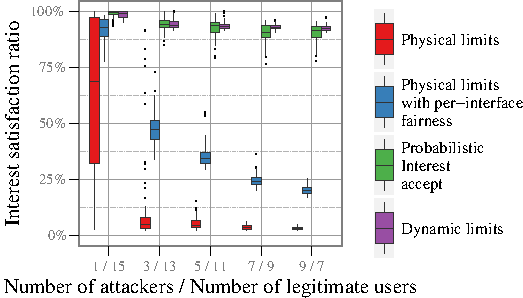
\includegraphics[scale=0.8]{paper-topo-tree/tree-good-0-producer-gw-avg-1-min}
  \caption{Average consumer Interest satisfaction ratios (first minute)}
  \label{fig:small-scale-topo boxplot}
\end{figure}

The presented results demonstrate the overall, and somewhat obvious, trends for all attack mitigation algorithms: the larger is the attack, the lower service quality is observed by the legitimate users.
Physical limits with and without per-interface fairness give perfect attack instrument even for a small number of attackers: just 3 attackers can either completely shut down or halve the service quality for the rest 13 users.
At the same time, while both intelligent attack mitigation algorithms also show a decline in service quality, this decline is very subtle: when more than 50\% of users are compromised, service degrades less than by 25\% for the satisfaction-based Interest accept method and less than by 10\% in the satisfaction-based pushback algorithm.


% \begin{figure}[htbp]
%   \centering
%   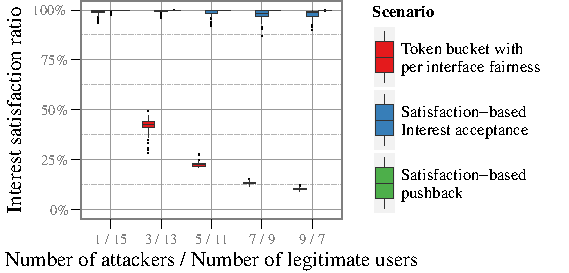
\includegraphics[scale=0.9]{tree-topo-var-evils-max-consumers-30mins/tree-good-0-producer-gw-avg-1-min-after-1-min}
%   \caption{Average consumer Interest satisfaction ratios (second minute)}
%   \label{fig:small-scale-topo 2}
% \end{figure}


%%% Local Variables: 
%%% mode: latex
%%% TeX-master: "paper"
%%% End: 
